%**************************************************************************
%*  Label-efficient land-use classification on EuroSAT                    *
%*  Team 21 - Deep Learning course project (P21)                          *
%*  Format: ELECTRONIC LETTERS ON COMPUTER VISION AND IMAGE ANALYSIS      *
%*          (LaTeX 2e template provided by the course instructor)         *
%**************************************************************************
%  Upload this file to the Overleaf copy of the ELCVIA template (it replaces
%  Elcvia2e.tex) together with all fig_*.png and tab_*.tex files.

\documentclass[twoside,a4paper,11pt]{article}
\usepackage{times}
\usepackage{elcvia}
\usepackage[english]{babel}
\usepackage{graphicx}

\newcommand{\Runo}{\rm I\hspace{-0.55ex}R}

\input{psfig.sty}
%\psdraft

% marks numbers that are still to be filled in (search for TBD before submitting)
\newcommand{\tbd}[1]{\textbf{[TBD: #1]}}
% number of trained networks: 72 (RGB grid) + 90 (first band run) + 36 (corrected band groups)
\newcommand{\nruns}{198}

% INFORMATION TO FILL IN CAMERA READY VERSION
%------------------------------------------------------------------
\newcommand{\vol}{0}      % Number of Volume (default 0)
\newcommand{\num}{0}      % Number (default 0)
\setcounter{page}{1}      % First page (default 1)
\newcommand{\begpag}{\thepage}
\newcommand{\finpag}{10}  % Last Page  (update to the real last page after compiling)
\newcommand{\yearp}{2026} % Year of the issue (default 2000)
%------------------------------------------------------------------
\renewcommand{\thefootnote}{\fnsymbol{footnote}}

\title{How Many Labels Do We Need? Label-Efficient Land-Use Classification
on EuroSAT with CNNs, ResNets and Vision Transformers
\footnote[0]{Correspondence to: $<$su-24029@sitare.org$>$ \vspace{0.2cm}}
%------------------------------------------------------------------
\footnote[0]{Deep Learning course project, Team 21 (project P21)}
%------------------------------------------------------------------
}

\author{Ishant Bhoyar$^*$, Ayush Kumar$^*$, Gaurav Kumar$^*$ and Jagriti Pandey$^*$ \\ \\
\centerline{\small \em $^*$ Sitare University, India} \\ \\
%------------------------------------------------------------------
\centerline{\small Deep Learning course project -- submitted November 2026}
       }


\begin{document}

\maketitle

\pagestyle{myheadings}

%------------------------------------------------------------------
\markboth{\centerline{\small \it Bhoyar et al. /
           Electronic Letters on Computer Vision and Image Analysis
           \vol(\num):\begpag-\finpag, \yearp}}
         {\centerline{\small \it Bhoyar et al. /
           Electronic Letters on Computer Vision and Image Analysis
           \vol(\num):\begpag-\finpag, \yearp}}
%------------------------------------------------------------------

\hrulefill

\begin{abstract}

Land-use maps are built from satellite images, but labelling those images
requires experts, so real projects have few labels. We study how much labelled
data is really needed on EuroSAT (27,000 Sentinel-2 patches, 10 classes).
We train a small CNN, a ResNet-50 and a ViT-S/16, from scratch and from ImageNet
weights, using 1\% to 100\% of the training labels, with three random seeds per
setting and one fixed test set. Pre-training is the strongest lever: with only
216 labelled images (1\%) the ImageNet ViT-S reaches 90.6\% and the ImageNet
ResNet-50 88.3\% accuracy, against 76.3\% for the small CNN and 73.5\% for a
ResNet-50 trained from scratch; the CNN needs about 3.6 to 5 times more labels to
match them. With all labels the gap closes (98.5\%--98.8\%) and differences are within
test-set noise. We also compare input bands using the 13-band version of
the data. Infrared bands help mostly when labels are scarce (about +2 to +3 points at 1\% of
the labels, almost nothing from 5\%), whereas feeding all
13 bands to a pre-trained network does not help. We report per-class errors
(highway/river and crop/vegetation confusions dominate), calibration, and a
band-order pitfall in the data files that we found and corrected.

\vspace{0.5cm}
\noindent
{\em Key Words}: Land-use classification, EuroSAT, Sentinel-2,
label efficiency, transfer learning, Vision Transformer, multispectral imagery.

\end{abstract}
\hrulefill

%------------------------------------------------------------------
\section{Introduction}

Satellite images are used to map cities, farmland, forests and water. Deep
networks classify such images very well when thousands of labelled examples
are available, but in practice labels are the bottleneck: an expert must look at every
patch. A practical question follows: \emph{given a fixed labelling budget, which
model and which training strategy should we choose, and do the extra spectral
bands of modern satellites change the answer?}

We study this question on EuroSAT [1], a benchmark of 27,000 Sentinel-2 patches of
$64\times64$ pixels in 10 land-use classes. Instead of reporting a single
accuracy with all labels, we simulate label scarcity by using only 1\%, 2\%, 5\%,
10\%, 25\% or 100\% of the training labels, and we draw
\emph{label-efficiency curves}. Our contributions are:

\begin{itemize}
\item A controlled study with one fixed split, class-balanced and nested label subsets,
three seeds per point, and a test set that is used once per run.
\item A comparison of three model families (small CNN, ResNet-50, ViT-S/16), each from
scratch and from ImageNet weights, under an identical training recipe.
\item A band ablation on the 13-band version of EuroSAT: which spectral bands help,
and at which label budgets.
\item An error and calibration analysis, and a report of a band-order pitfall in the
EuroSAT multispectral files.
\end{itemize}

%------------------------------------------------------------------
\section{Related Work}

\textbf{Land-use benchmarks.} EuroSAT [1] provides Sentinel-2 patches in an RGB
and a 13-band version; its authors reported 98.57\% accuracy with a fine-tuned
ResNet-50. BigEarthNet [2] is a larger multi-label Sentinel-2 benchmark. Surveys
such as [3] describe the growing use of deep learning in remote sensing.

\textbf{Transfer learning.} Fine-tuning networks pre-trained on ImageNet [4] is the
standard way to cope with few labels; whether better ImageNet models transfer better
is studied in [5]. Remote-sensing-specific pre-training can help further [6]; we do not
use it, and only ImageNet weights are used here.

\textbf{Architectures.} ResNets [7] use skip connections to train deep convolutional
networks. Vision Transformers [8] split an image into patches and use attention;
they need large amounts of data when trained from scratch, and the augmentation and
regularisation used in pre-training matter a lot [9]. We use the ImageNet-21k
pre-trained ViT-S/16 weights released through the \texttt{timm} library [10].

%------------------------------------------------------------------
\section{Dataset and Experimental Protocol}

\subsection{EuroSAT}

EuroSAT [1] contains 27,000 labelled patches from Sentinel-2 [11] (10~m resolution,
$64\times64$ pixels) over European countries, in 10 classes: AnnualCrop, Forest,
HerbaceousVegetation, Highway, Industrial, Pasture, PermanentCrop, Residential,
River and SeaLake (2,000--3,000 images per class). It is distributed as an RGB version
(8-bit JPEG) and as a multispectral version with all 13 Sentinel-2 bands (16-bit GeoTIFF).
Figure~\ref{fig:samples} shows examples; the visual similarity between several
classes (e.g.\ Pasture, HerbaceousVegetation and PermanentCrop, or Highway and River)
already suggests where errors will occur.

\begin{figure}[t]
\centering
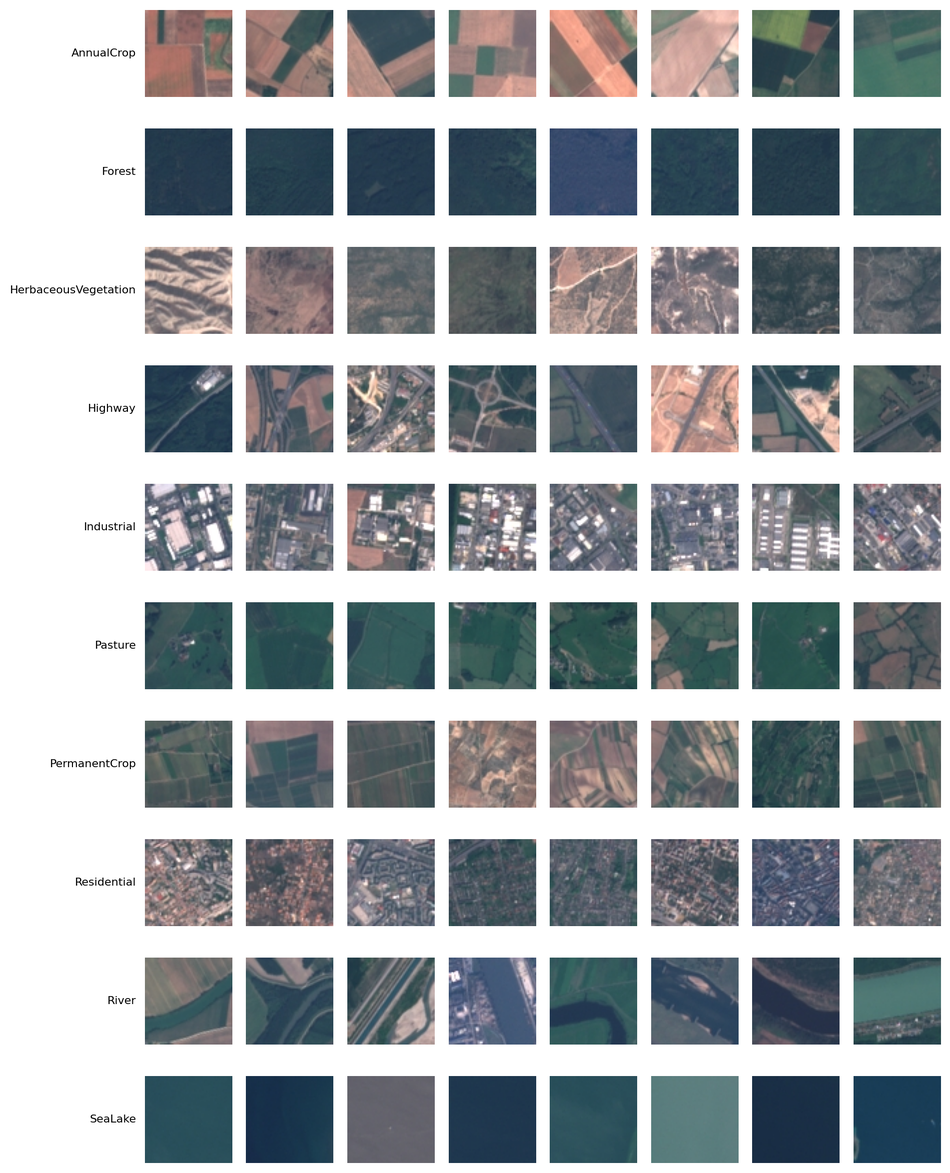
\includegraphics[width=0.52\linewidth]{fig_samples.png}
\caption{Random EuroSAT examples (RGB), one row per class: AnnualCrop, Forest,
HerbaceousVegetation, Highway, Industrial, Pasture, PermanentCrop, Residential, River, SeaLake.}
\label{fig:samples}
\end{figure}

\subsection{Split and label budgets}

We create \emph{one} stratified split, with seed 0, of 80\% training (21,600
images), 10\% validation (2,700) and 10\% test (2,700). The same image
identifiers are used for the RGB and the 13-band versions, so that comparisons between
input bands use exactly the same images. To simulate scarce labels we keep
a class-balanced subset of the \emph{training} set: 1\% (216 images, 22 per class),
2\%, 5\%, 10\%, 25\% or 100\%. For a given seed the subsets are nested (the 1\%
subset is contained in the 2\% subset, and so on), so a learning curve changes only the
amount of data and not which images were drawn. Different seeds give different subsets
and different initialisations. Validation images are used only to choose the
checkpoint; the test set is used once per run for the reported numbers.

\subsection{Metrics}

We report test accuracy (mean and standard deviation over three seeds) and macro-averaged F1
score. For error analysis we use per-class F1, row-normalised confusion matrices, and the
Expected Calibration Error (ECE, 15 bins) [12].

%------------------------------------------------------------------
\section{Methods}

\subsection{Models}

\textbf{Small CNN.} Four stages of two $3\times3$ convolutions (BatchNorm, ReLU)
followed by max-pooling, with 32/64/128/256 channels, global average pooling and a linear
classifier (about 1.2 M parameters). It is trained from scratch and is our baseline.

\textbf{ResNet-50.} The standard 50-layer residual network [7], either with random
initialisation (scratch) or initialised from ImageNet weights [4] (``ImageNet'').

\textbf{ViT-S/16.} A Vision Transformer-Small with $16\times16$ patches [8], initialised from
the ImageNet-21k pre-trained and ImageNet-1k fine-tuned weights of [9]; the position
embeddings are resampled to the input size.

Images are up-sampled from $64\times64$ to $112\times112$ for ResNet-50 and ViT-S;
the small CNN uses $64\times64$. For pre-trained models with more than three input channels,
the first layer is adapted by re-using the pre-trained RGB filters for the extra channels
(the default of \texttt{timm}).

\subsection{Training recipe}

All models use the same recipe, so differences come from the model and not from
tuning. We use AdamW [13] with weight decay 0.05, a learning rate of $10^{-3}$ for models trained
from scratch and $3\cdot10^{-4}$ for pre-trained models, 5\% linear warm-up followed by cosine decay,
cross-entropy with label smoothing 0.1 [14], batch size 128 and mixed precision. Inputs are
standardised with per-channel statistics. Augmentation consists of random
rotations by multiples of 90$^\circ$ and flips, which is natural for overhead imagery. Because one
epoch on a tiny subset is only one or two updates, every run performs at least 600 weight
updates (otherwise 20 epochs, 40 for the small CNN). The checkpoint with the best validation accuracy
(evaluated about 20 times per run) is tested. In total we trained \nruns{} networks
on Kaggle T4 GPUs; one run takes from about 15~seconds (CNN, 1\% of labels) to about 9~minutes
(ResNet-50, all labels).

\subsection{Band ablation}

For the multispectral experiments we use the 13-band files and an ImageNet-pre-trained
ResNet-50, and feed only a subset of the bands (always starting with R,G,B so that the
pre-trained RGB filters see RGB): (i) R,G,B only, taken from the 13-band files; (ii) adding the
near-infrared band B08; (iii) adding B08 and the red-edge bands B05, B06, B07 and the narrow
NIR band B8A; (iv) adding B08 and the short-wave infrared bands B11 and B12; and (v) all 13 bands.
The reference for gains is setting (i), not the JPEG RGB images, because the JPEGs were
produced with a different radiometric processing (Section~\ref{sec:rgbvs}).

\paragraph{A band-order pitfall.} We first assumed that the 13 channels of the GeoTIFF files follow
the order B01--B08, B8A, B09--B12 given in the documentation. The spectral
signatures we plotted (Figure~\ref{fig:spectral}) contradict this: channel 9 is almost zero
for every class, as expected for the cirrus band B10, and channel 12 follows the NIR band B08
(bright for crops, dark for water), as expected for B8A. The files therefore store the bands as
B01--B08, B09, B10, B11, B12, B8A, i.e.\ B8A \emph{last}. Our first ablation run had used the
documented order, so its two ``extended'' groups contained other bands than their names stated
(they were B08+B12+B8A and B08+B05--B07+B09). We report these two runs
under their true band lists, fixed the code, and re-ran the intended groups (iii) and (iv).

\begin{figure}[t]
\centering
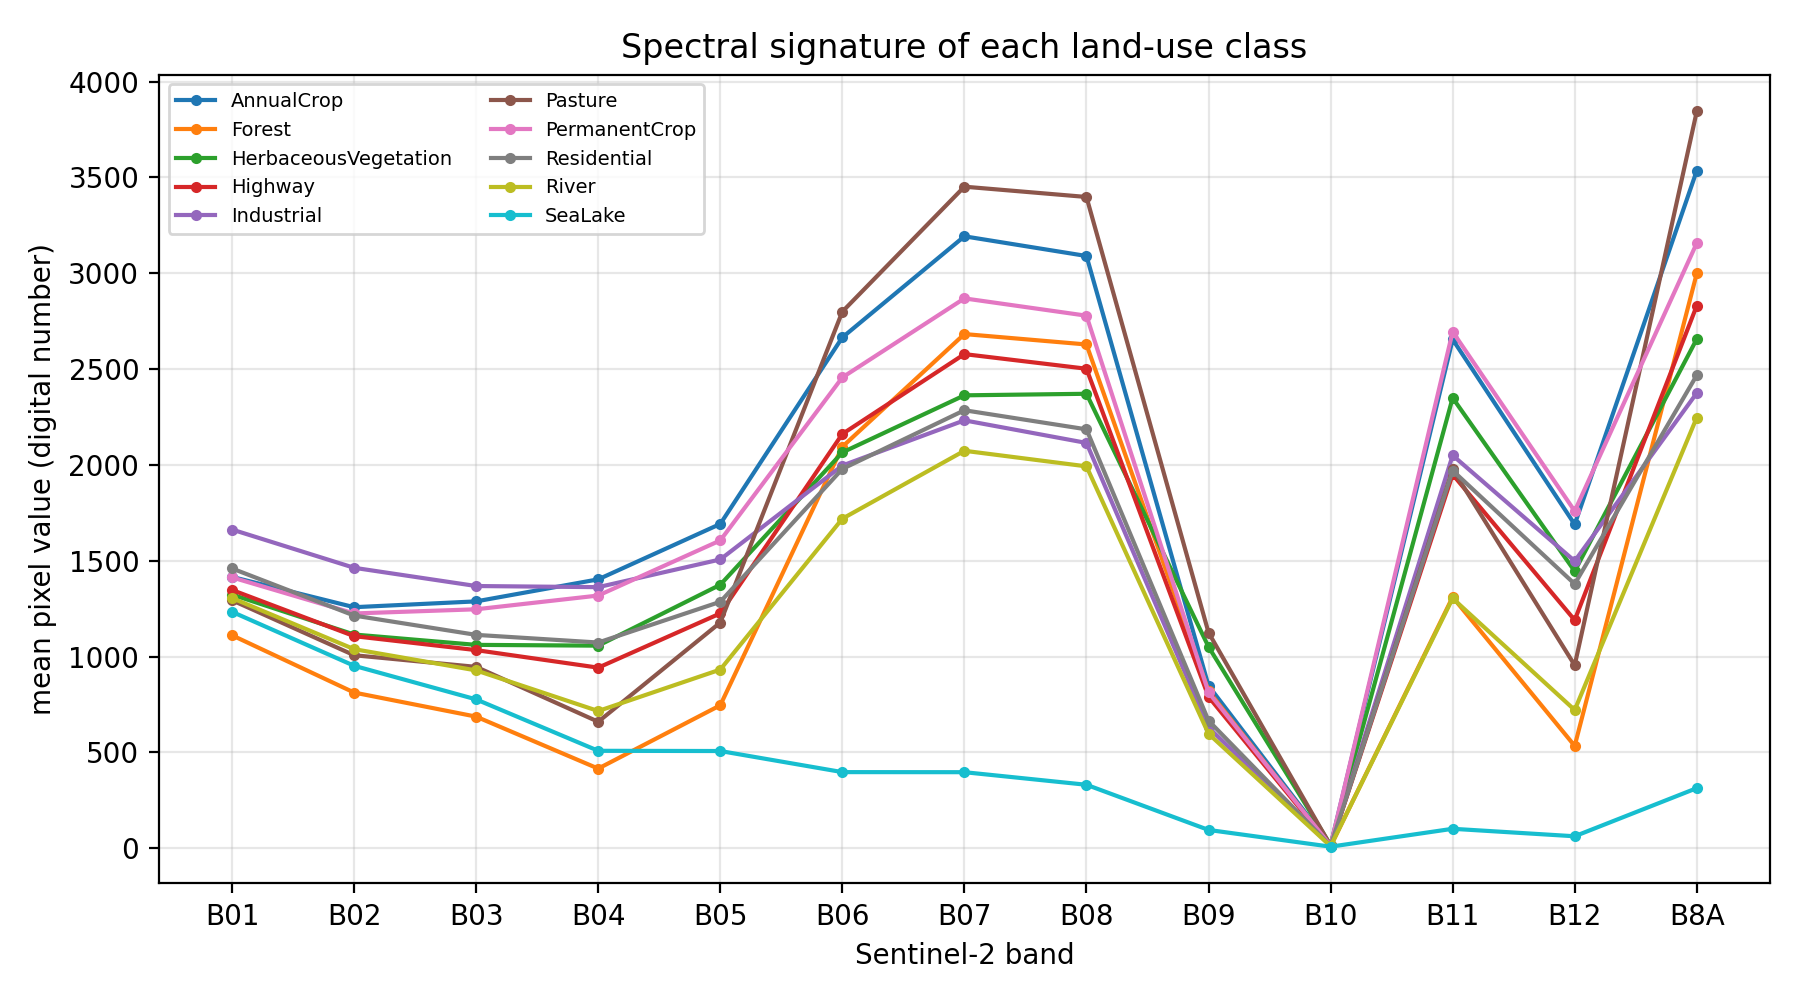
\includegraphics[width=0.92\linewidth]{fig_spectral.png}
\caption{Mean value of each channel of the 13-band files (training set) for each class.
Band names on the horizontal axis follow the \emph{verified} channel order, in which B8A is stored last.
Water (SeaLake) has almost no signal in the infrared channels, and vegetation classes are bright in the
near-infrared and red-edge channels.}
\label{fig:spectral}
\end{figure}

%------------------------------------------------------------------
\section{Results}

\subsection{Label efficiency}

Table~\ref{tab:main} and Figure~\ref{fig:labeleff} show the main result.

\begin{figure}[t]
\centering
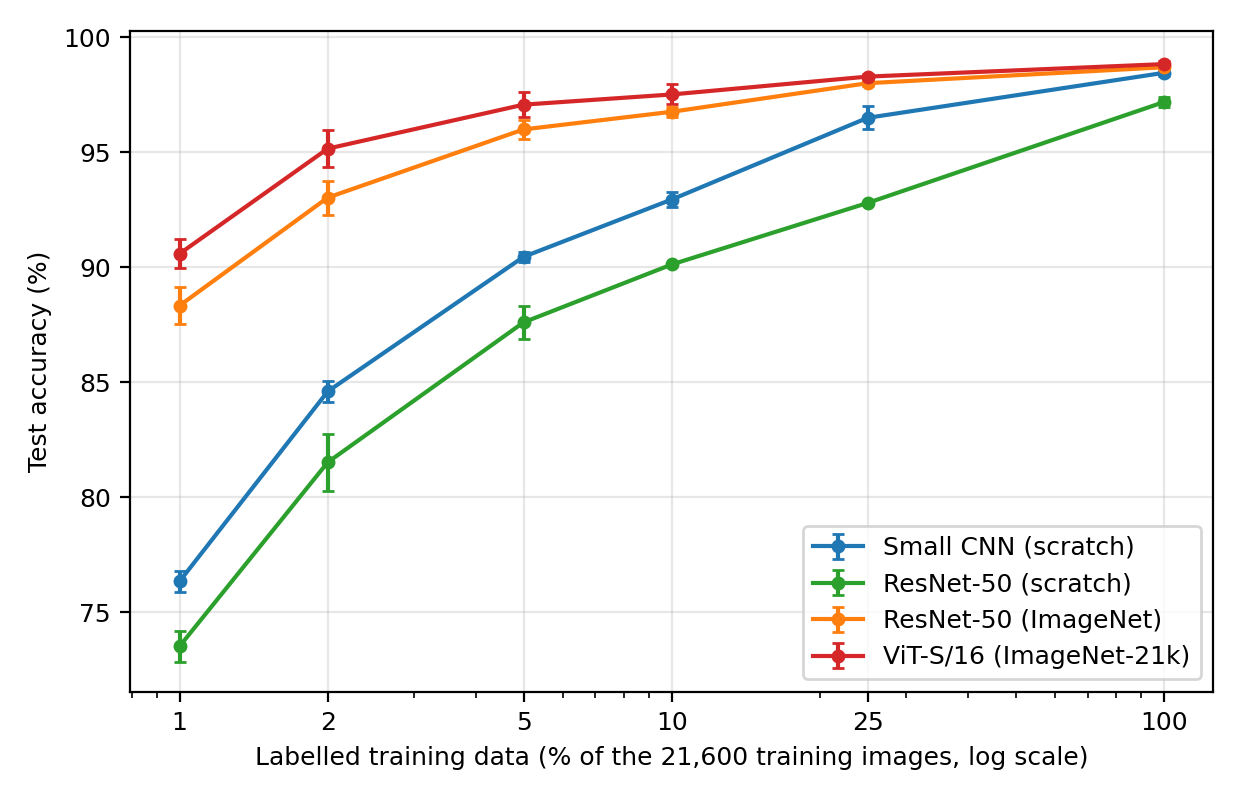
\includegraphics[width=0.82\linewidth]{fig_label_eff.png}
\caption{Label-efficiency curves on EuroSAT RGB. Points are means over three seeds and
bars are standard deviations. The horizontal axis is logarithmic.}
\label{fig:labeleff}
\end{figure}

\begin{table}[t]
\centering
\small
\setlength{\tabcolsep}{4pt}
\begin{tabular}{|l|c|c|c|c|c|c|}
\hline
Model / input & 1\% & 2\% & 5\% & 10\% & 25\% & 100\% \\ \hline \hline
Small CNN (scratch) & 76.3 $\pm$ 0.5 & 84.6 $\pm$ 0.4 & 90.5 $\pm$ 0.2 & 93.0 $\pm$ 0.3 & 96.5 $\pm$ 0.5 & 98.5 $\pm$ 0.1 \\
ResNet-50 (scratch) & 73.5 $\pm$ 0.7 & 81.5 $\pm$ 1.2 & 87.6 $\pm$ 0.7 & 90.1 $\pm$ 0.1 & 92.8 $\pm$ 0.1 & 97.2 $\pm$ 0.2 \\
ResNet-50 (ImageNet) & 88.3 $\pm$ 0.8 & 93.0 $\pm$ 0.7 & 96.0 $\pm$ 0.4 & 96.8 $\pm$ 0.2 & 98.0 $\pm$ 0.1 & 98.7 $\pm$ 0.1 \\
ViT-S/16 (ImageNet-21k) & \textbf{90.6 $\pm$ 0.6} & \textbf{95.2 $\pm$ 0.8} & \textbf{97.1 $\pm$ 0.5} & \textbf{97.5 $\pm$ 0.4} & \textbf{98.3 $\pm$ 0.1} & \textbf{98.8 $\pm$ 0.1} \\
\hline
\end{tabular}
\caption{Test accuracy (\%, mean $\pm$ std over 3 seeds) on EuroSAT RGB for different percentages of the 21,600 labelled training images (1\% = 216 images). Best value per column in bold.}
\label{tab:main}
\end{table}

\textbf{Pre-training is the strongest lever.} With 216 labelled images (1\%, about 22 per class),
the ImageNet ViT-S reaches 90.6\% and the ImageNet ResNet-50 88.3\%, while the small CNN reaches
76.3\% and ResNet-50 trained from scratch 73.5\%. Interpolating the CNN curve on a logarithmic
label axis, the CNN needs about 3.6\% of the labels (about 770 images) to match the ImageNet
ResNet-50 at 1\%, and about 5.2\% (about 1,120 images) to match the ViT-S: pre-training is worth a
factor of about 3.6 to 5 in labels at this operating point.

\textbf{The ViT-S is the best RGB model when labels are scarce.} Its advantage over the ImageNet
ResNet-50 is $+2.3$ points at 1\%, $+2.2$ at 2\%, $+1.1$ at 5\%, $+0.7$ at 10\%, $+0.3$ at 25\% and $+0.1$ at 100\%.
The seed-to-seed standard deviation is at most 1.2 points, so the gaps at 1--5\% are clear, whereas
at 25\% and 100\% they are not.

\textbf{More capacity does not help without pre-training.} ResNet-50 from scratch is worse than the small
CNN at every label budget ($-2.8$ points at 1\%, $-3.7$ at 25\%, $-1.3$ at 100\%): a 23.5 M-parameter
network overfits a few hundred images.

\textbf{With all labels the models converge.} At 100\% the three good models reach 98.5\%, 98.7\% and 98.8\%.
With 2,700 test images, the 95\% sampling uncertainty of an accuracy of 98.7\% is about $\pm0.4$ points,
so these three models cannot be separated. Label efficiency, not final accuracy, is what distinguishes the methods.

\subsection{Effect of spectral bands}

\begin{table}[t]
\centering
\small
\setlength{\tabcolsep}{4pt}
\begin{tabular}{|l|c|c|c|c|c|c|}
\hline
Input bands & 1\% & 2\% & 5\% & 10\% & 25\% & 100\% \\ \hline \hline
R,G,B & 89.4 $\pm$ 0.6 & 93.7 $\pm$ 0.1 & 96.4 $\pm$ 0.2 & 97.3 $\pm$ 0.1 & 98.0 $\pm$ 0.0 & 98.8 $\pm$ 0.1 \\
R,G,B + B08 (NIR) & 91.4 $\pm$ 0.3 & 94.7 $\pm$ 0.4 & 96.7 $\pm$ 0.5 & 97.1 $\pm$ 0.1 & 98.1 $\pm$ 0.3 & 98.9 $\pm$ 0.1 \\
R,G,B + B08 + B05,B06,B07,B8A (red-edge) & 91.8 $\pm$ 0.8 & 95.0 $\pm$ 0.5 & 96.5 $\pm$ 0.3 & 97.4 $\pm$ 0.3 & 98.1 $\pm$ 0.1 & 99.2 $\pm$ 0.1 \\
R,G,B + B08 + B11,B12 (SWIR) & 92.2 $\pm$ 0.9 & 95.0 $\pm$ 0.2 & \textbf{96.8 $\pm$ 0.2} & \textbf{97.5 $\pm$ 0.1} & 98.0 $\pm$ 0.2 & 99.0 $\pm$ 0.1 \\
R,G,B + B08 + B12,B8A (first run) & \textbf{92.3 $\pm$ 0.3} & \textbf{95.2 $\pm$ 0.6} & 96.7 $\pm$ 0.2 & 97.5 $\pm$ 0.2 & \textbf{98.2 $\pm$ 0.1} & \textbf{99.2 $\pm$ 0.1} \\
R,G,B + B08 + B05--B07,B09 (first run) & 90.8 $\pm$ 0.2 & 94.7 $\pm$ 0.4 & 96.6 $\pm$ 0.4 & 97.2 $\pm$ 0.3 & 98.1 $\pm$ 0.1 & 98.9 $\pm$ 0.2 \\
All 13 bands & 89.2 $\pm$ 0.6 & 93.4 $\pm$ 0.9 & 95.7 $\pm$ 0.3 & 96.8 $\pm$ 0.4 & 98.0 $\pm$ 0.1 & 98.9 $\pm$ 0.2 \\
\hline
\end{tabular}
\caption{Band ablation with an ImageNet-pre-trained ResNet-50 (test accuracy \%, mean $\pm$ std over 3 seeds). All inputs come from the 13-band files. B02, B03, B04 = blue, green, red; B08 = near-infrared; B05--B07 and B8A = red-edge/narrow NIR; B11, B12 = short-wave infrared. The two ``first run'' rows are band sets that were run before we discovered that the band order in the files differs from the documentation (see text).}
\label{tab:bands}
\end{table}

\begin{figure}[t]
\centering
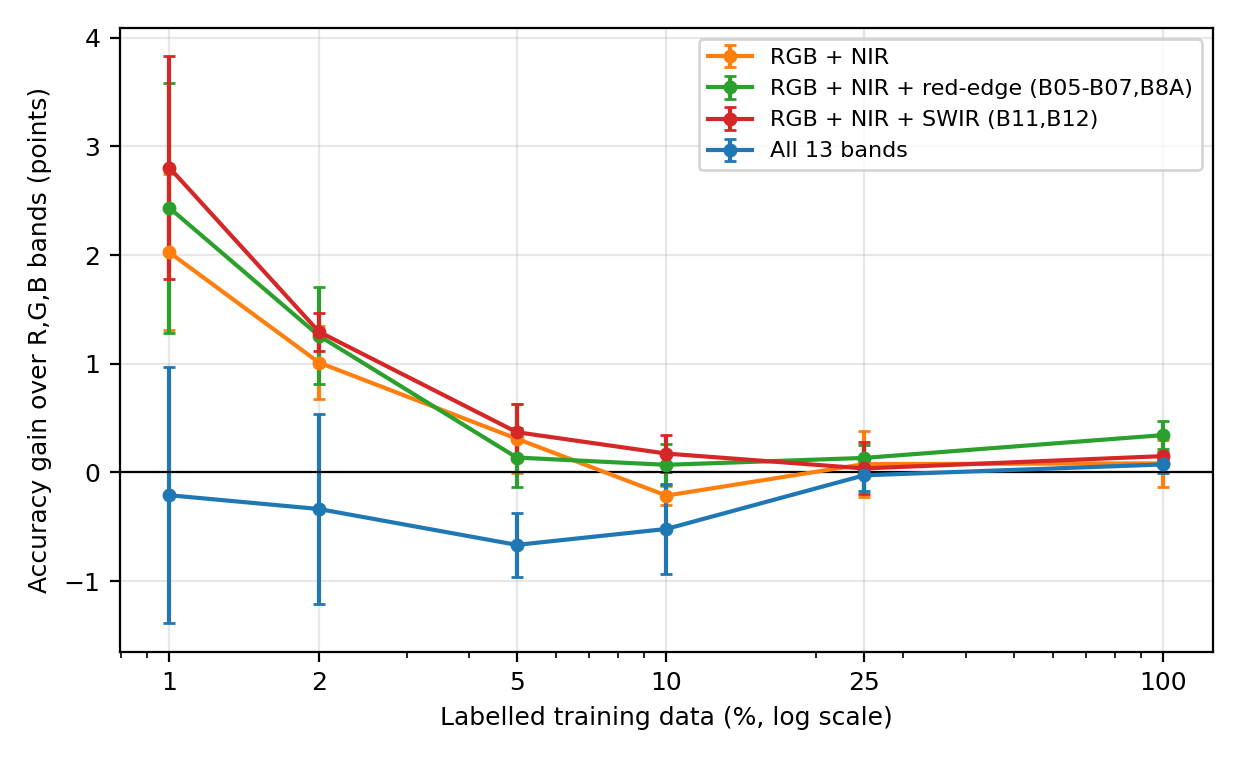
\includegraphics[width=0.82\linewidth]{fig_bands.png}
\caption{Accuracy gain of extra bands over R,G,B (taken from the same 13-band files), paired by seed
(mean and standard deviation of the three paired differences), for the ImageNet ResNet-50.}
\label{fig:bands}
\end{figure}

Table~\ref{tab:bands} and Figure~\ref{fig:bands} give the ablation. Differences between inputs are small compared
with the differences between models, but they have a clear pattern.

\textbf{Near-infrared helps when labels are scarce.} Adding B08 gives $+2.0\pm0.7$ points at 1\% of the labels and
$+1.0\pm0.3$ at 2\%, and nothing measurable from 5\% on. Infrared reflectance separates vegetation from
built-up and water surfaces (Figure~\ref{fig:spectral}), information that a network with few examples cannot easily
extract from the visible bands alone.

\textbf{More bands is not better.} Feeding all 13 bands to the pre-trained network is slightly worse than R,G,B for
1--10\% of the labels ($-0.2$ to $-0.7$ points; at 1--2\% this is within one standard deviation, at 5--10\% it is not)
and equal at 25--100\% ($0.0$ and $+0.1$). A likely reason is that the pre-trained
first layer was learned for three channels, and ten extra channels dilute it; with few labels the network cannot
relearn it. Selecting a few informative bands is better than using all of them (at 1\%, 91.4--92.3\% against 89.2\%).

\textbf{Beyond near-infrared.} The corrected groups give $+2.4\pm1.2$ points at 1\% of the labels for the red-edge set
(B05--B07, B8A) and $+2.8\pm1.0$ for the SWIR set (B11, B12), against $+2.0\pm0.7$ for B08 alone; at 2\% both give $+1.3$
against $+1.0$. The extra gain over B08 alone (at most 0.8 points) is smaller than the seed-to-seed standard deviation, so
with three seeds we cannot rank the NIR-only, red-edge and SWIR inputs. From 5\% of the labels on, every group is
within $\pm0.4$ points of R,G,B, which is the resolution of the test set.

\textbf{The first-run band sets.} The set B08+B12+B8A has the highest mean at 1\% ($92.3\pm0.3$\%, $+2.9\pm0.9$ points over
R,G,B) and at 100\% ($99.2\pm0.1$\%, $+0.4\pm0.0$), but it is statistically tied with the corrected SWIR set ($92.2\pm0.9$\% at 1\%), which
shares the band B12, and with the corrected red-edge set at 100\%. B08+B05--B07+B09 gave the smallest gain of the extended
sets ($+1.5\pm0.8$ at 1\%), possibly because B09 (water vapour) carries little information about the land surface.

\subsection{JPEG RGB versus RGB from the multispectral files}
\label{sec:rgbvs}

The ImageNet ResNet-50 on the JPEG RGB images (Table~\ref{tab:main}) is slightly worse than on the same three
bands taken from the 13-band files (Table~\ref{tab:bands}): $-1.1$ points at 1\%, $-0.7$ at 2\%, $-0.4$ at 5\%
and $-0.1$ at 100\%. The JPEGs are 8-bit images with a different contrast stretch, while the GeoTIFFs keep the
16-bit reflectance values. This is why all band comparisons use the 13-band R,G,B as their reference.

\subsection{Error analysis}

\begin{figure*}[t]
\centering
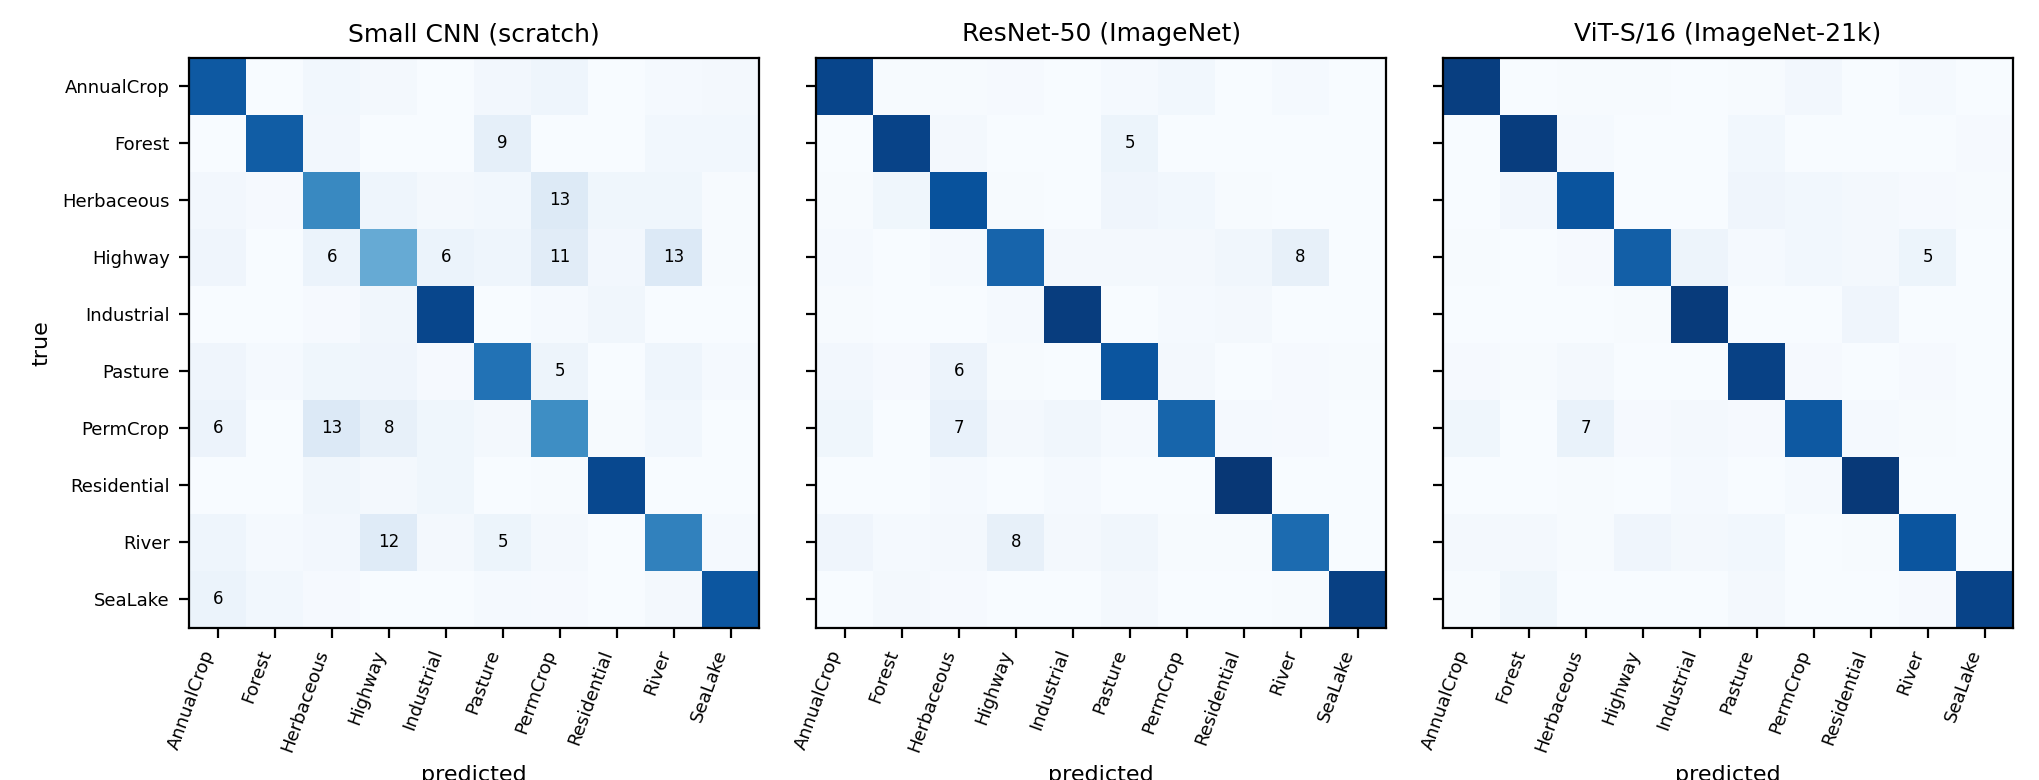
\includegraphics[width=\linewidth]{fig_confusion.png}
\caption{Row-normalised confusion matrices at 1\% of the labels, summed over three seeds. Off-diagonal cells
above 5\% are annotated (in \%). Rows are true classes, columns are predictions.}
\label{fig:confusion}
\end{figure*}

\begin{table}[t]
\centering
\small
\setlength{\tabcolsep}{5pt}
\begin{tabular}{|l|c|c|c|c|}
\hline
Class & CNN & R50 scratch & R50 ImageNet & ViT-S \\ \hline \hline
AnnualCrop & 81.1 & 79.4 & 90.4 & \textbf{93.5} \\
Forest & 87.6 & 85.5 & 91.9 & \textbf{93.3} \\
HerbaceousVegetation & 66.9 & 64.0 & 84.6 & \textbf{87.4} \\
Highway & 54.1 & 45.7 & 82.4 & \textbf{87.1} \\
Industrial & 86.3 & 86.3 & \textbf{92.9} & 92.1 \\
Pasture & 70.2 & 69.1 & 80.4 & \textbf{87.1} \\
PermanentCrop & 62.1 & 63.7 & 82.7 & \textbf{85.6} \\
Residential & 90.4 & 85.3 & \textbf{95.3} & 94.2 \\
River & 68.3 & 63.1 & 81.5 & \textbf{87.5} \\
SeaLake & 88.2 & 83.7 & \textbf{96.1} & 95.1 \\
\hline Macro average & 75.5 & 72.6 & 87.8 & 90.3 \\ \hline
\end{tabular}
\caption{Per-class F1 score (\%) on the test set when only 1\% of the labels (about 22 images per class) are used, averaged over 3 seeds. Best value per class in bold.}
\label{tab:f1}
\end{table}

Figure~\ref{fig:confusion} and Table~\ref{tab:f1} analyse the 1\% setting. The dominant confusions are
\emph{Highway $\leftrightarrow$ River} (8\% in both directions for the ImageNet ResNet-50, 13\% and 12\% for
the small CNN): both are thin, elongated, linear structures crossing other land cover.
The second group is \emph{PermanentCrop $\rightarrow$ HerbaceousVegetation} (7.5\%) and
\emph{Pasture $\rightarrow$ HerbaceousVegetation} (5.8\%): the three are textured green/brown surfaces.
ResNet-50 from scratch is the extreme case with a Highway F1 of only 45.7\%. Pre-trained models are
better in every class, and the ViT-S is the best or tied in most classes. The classes that are easy for every model
are SeaLake, Residential, Forest and Industrial. With all labels the same pairs remain the
largest errors but are much smaller (Pasture $\rightarrow$ HerbaceousVegetation 2.0\%, River
$\rightarrow$ Highway 1.6\%, PermanentCrop $\rightarrow$ HerbaceousVegetation 1.5\% for the ImageNet ResNet-50).

\subsection{Calibration}

\begin{table}[t]
\centering
\small
\setlength{\tabcolsep}{4pt}
\begin{tabular}{|l|ccc|ccc|}
\hline
 & \multicolumn{3}{c|}{1\% of labels} & \multicolumn{3}{c|}{100\% of labels} \\
Model & acc. & conf. & ECE & acc. & conf. & ECE \\ \hline \hline
CNN & 76.3 & 76.1 & 2.9 & 98.5 & 88.9 & 9.6 \\
R50 scratch & 73.5 & 71.6 & 3.3 & 97.2 & 88.2 & 9.0 \\
R50 ImageNet & 88.3 & 76.5 & 11.9 & 98.7 & 90.1 & 8.9 \\
ViT-S & 90.6 & 80.4 & 10.3 & 98.8 & 90.5 & 8.7 \\
\hline
\end{tabular}
\caption{Calibration on the test set: accuracy, mean confidence and Expected Calibration Error (all in \%, 15 bins), averaged over 3 seeds. Training used label smoothing 0.1; no post-hoc calibration was applied.}
\label{tab:ece}
\end{table}

Table~\ref{tab:ece} shows that all models are \emph{under}-confident, not over-confident:
with all labels the mean confidence is 88--91\% while the accuracy is 97--99\%, an ECE of about 9\%.
At 1\% of the labels the pre-trained models are the most under-confident (ECE 10--12\%) and the
models from scratch are almost calibrated (ECE about 3\%). We attribute this to label smoothing
[14], which caps the confidence the network is trained to produce [15]. If calibrated probabilities are needed,
post-hoc temperature scaling should be added; we did not apply it.

%------------------------------------------------------------------
\section{Discussion}

\textbf{Practical recommendation.} For a land-use task with a small labelling budget, start from a pre-trained
model: this is worth the same accuracy as 3.6 to 5 times more labels, much more than any architectural choice or
input-band choice we tried. A ViT-S/16 is a good default at 1--5\% of the labels; with a quarter of the labels or more a pre-trained
ResNet-50 is within 0.3 points of it, and even a small CNN trained from scratch is within 0.3 points
at 100\% of the labels. When labels are very scarce and infrared bands are available, feeding a small, well-chosen
set of them (rather than all bands) gives an additional gain of about 2 to 3 points at 1\% of the labels. Most of it
comes from the single near-infrared band; adding red-edge or SWIR bands on top changes the result by less than the seed noise.
From 5\% of the labels on, the gain is below 0.5 points.

\textbf{Limitations.} (1) EuroSAT patches come from the same scenes, and we split patches at random,
so patches from neighbouring locations can be in both the training and the test set; absolute accuracies are
therefore optimistic, although all methods are compared on the same split. A spatially disjoint split would
be a harder and more realistic test. (2) We use one split and three seeds; the seeds vary the label
subset and the initialisation but not the test set, and the 2,700 test images limit the resolution to
about $\pm0.4$ points near 98.7\%. (3) We used one hyper-parameter recipe for all models; per-model tuning could change
the gaps, especially for the ViT. (4) Images were up-sampled to 112 pixels for the large models, which is
cheap but not necessarily optimal. (5) The band study uses one architecture, and the extra bands are fed through
a first layer that was pre-trained on RGB. (6) We did not explore self-supervised or semi-supervised
learning, nor remote-sensing-specific pre-trained models [6], which are natural next steps for the low-label regime.

%------------------------------------------------------------------
\section{Conclusion}

On EuroSAT, the amount of labelled data needed depends mostly on whether the network is pre-trained: with 22 labelled
images per class an ImageNet-pre-trained ViT-S reaches 90.6\% accuracy and ResNet-50 88.3\%, against 76.3\% for a
small CNN, and a CNN needs 3.6 to 5 times more labels to catch up; with all labels every good model is at 98.5--98.8\%.
Near-infrared information adds about 2 points when only 1\% of the labels are available (2.4--2.9 points with red-edge or
short-wave-infrared bands as well, a difference within noise) and almost nothing from 5\% of the labels on,
while using all 13 bands with a pre-trained network does not help. Most errors are between visually similar
classes (Highway/River and the crop/vegetation group), and all models are under-confident because of label smoothing.
We also found that the band order of the EuroSAT multispectral files differs from its documentation, which silently
changes what a ``NIR'' or ``SWIR'' ablation contains. The code, the split and the results are available at
github.com/kumarAyush24029/Eurosat-label-efficiency.

%------------------------------------------------------------------
\begin{thebibliography}{99}

\bibitem{Hel:19}
P. Helber, B. Bischke, A. Dengel, D. Borth,
``EuroSAT: A novel dataset and deep learning benchmark for land use and land cover classification'',
{\em IEEE Journal of Selected Topics in Applied Earth Observations and Remote Sensing} 12(7):2217-2226, 2019.

\bibitem{Sum:19}
G. Sumbul, M. Charfuelan, B. Demir, V. Markl,
``BigEarthNet: A large-scale benchmark archive for remote sensing image understanding'',
{\em IEEE Intl. Geoscience and Remote Sensing Symposium (IGARSS)}, 5901-5904, 2019.

\bibitem{Zhu:17}
X. X. Zhu, D. Tuia, L. Mou, G.-S. Xia, L. Zhang, F. Xu, F. Fraundorfer,
``Deep learning in remote sensing: A comprehensive review and list of resources'',
{\em IEEE Geoscience and Remote Sensing Magazine} 5(4):8-36, 2017.

\bibitem{Den:09}
J. Deng, W. Dong, R. Socher, L.-J. Li, K. Li, L. Fei-Fei,
``ImageNet: A large-scale hierarchical image database'',
{\em IEEE Conf. on Computer Vision and Pattern Recognition (CVPR)}, 248-255, 2009.

\bibitem{Kor:19}
S. Kornblith, J. Shlens, Q. V. Le,
``Do better ImageNet models transfer better?'',
{\em IEEE Conf. on Computer Vision and Pattern Recognition (CVPR)}, 2661-2671, 2019.

\bibitem{Neu:19}
M. Neumann, A. S. Pinto, X. Zhai, N. Houlsby,
``In-domain representation learning for remote sensing'',
{\em arXiv:1911.06721}, 2019.

\bibitem{He:16}
K. He, X. Zhang, S. Ren, J. Sun,
``Deep residual learning for image recognition'',
{\em IEEE Conf. on Computer Vision and Pattern Recognition (CVPR)}, 770-778, 2016.

\bibitem{Dos:21}
A. Dosovitskiy, L. Beyer, A. Kolesnikov, D. Weissenborn, X. Zhai, T. Unterthiner, M. Dehghani,
M. Minderer, G. Heigold, S. Gelly, J. Uszkoreit, N. Houlsby,
``An image is worth 16x16 words: Transformers for image recognition at scale'',
{\em Intl. Conf. on Learning Representations (ICLR)}, 2021.

\bibitem{Ste:22}
A. Steiner, A. Kolesnikov, X. Zhai, R. Wightman, J. Uszkoreit, L. Beyer,
``How to train your ViT? Data, augmentation, and regularization in Vision Transformers'',
{\em Transactions on Machine Learning Research}, 2022.

\bibitem{Wig:19}
R. Wightman,
``PyTorch Image Models (timm)'',
{\em github.com/huggingface/pytorch-image-models}, 2019.

\bibitem{Dru:12}
M. Drusch et al.,
``Sentinel-2: ESA's optical high-resolution mission for GMES operational services'',
{\em Remote Sensing of Environment} 120:25-36, 2012.

\bibitem{Guo:17}
C. Guo, G. Pleiss, Y. Sun, K. Q. Weinberger,
``On calibration of modern neural networks'',
{\em Intl. Conf. on Machine Learning (ICML)}, 1321-1330, 2017.

\bibitem{Los:19}
I. Loshchilov, F. Hutter,
``Decoupled weight decay regularization'',
{\em Intl. Conf. on Learning Representations (ICLR)}, 2019.

\bibitem{Sze:16}
C. Szegedy, V. Vanhoucke, S. Ioffe, J. Shlens, Z. Wojna,
``Rethinking the Inception architecture for computer vision'',
{\em IEEE Conf. on Computer Vision and Pattern Recognition (CVPR)}, 2818-2826, 2016.

\bibitem{Mul:19}
R. M\"uller, S. Kornblith, G. Hinton,
``When does label smoothing help?'',
{\em Advances in Neural Information Processing Systems (NeurIPS)}, 2019.

\end{thebibliography}

\end{document}
